\section{Model definition}
\label{model-definition}
This Section presents how the networks used on the training set are 
structured and how the Hyperparameter tuning phase was performed.

\subsection{Neural network structure}
The starting point for the neural network structure was a 
reasonable network in terms of hidden neurons to prevent over-fitting, 
indeed a high number of units in the hidden layers would end up in learning 
too much from the dataset.

The rule of thumb followed to decide hidden neurons quantity is the 
following: 
$$\#\mathit{hidden\; neurons} = \frac{2}{3}\#\mathit{input\;neurons}
+ \#\mathit{output\;neurons}$$
The next step was to decide the hidden layer number. To respect the 
number of hidden neurons, two hidden layers were considered. 
A more complex structure in terms of layers number would mean 
having a real small number of neurons per layer.

To give reference, this is the model used on the PCA training set, mentioned at 
the end of Subsection \vref{extended-dataset}, with 
120 input features.

\begin{center}
    
    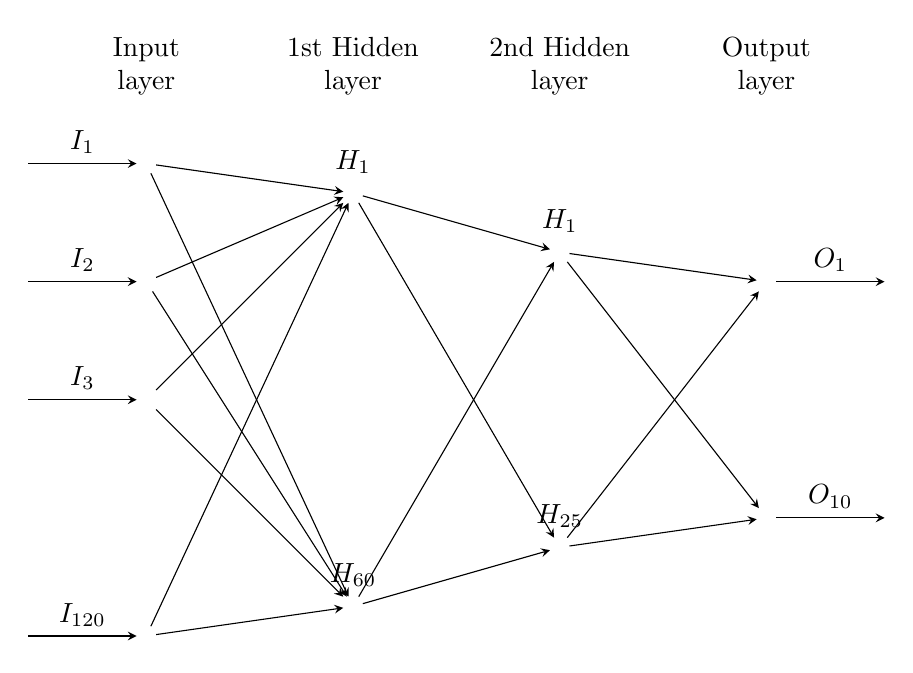
\begin{tikzpicture}[x=1.5cm, y=1.5cm, >=stealth]
        
        % layers
        \foreach \m/\l [count=\y] in {1,2,3,missing,4}
        \node [every neuron/.try, neuron \m/.try] (input-\m) at (0,2.5-\y) {};
        
        \foreach \m [count=\y] in {1,missing,2}
        \node [every neuron/.try, neuron \m/.try ] (hidden-\m) at (1.75,3-\y*1.75) {};
        
        \foreach \m [count=\y] in {1,missing,2}
        \node [every neuron/.try, neuron \m/.try ] (hidden2-\m) at (3.5,2-\y*1.25) {};
        
        \foreach \m [count=\y] in {1,missing,2}
        \node [every neuron/.try, neuron \m/.try ] (output-\m) at (5.25,1.5-\y) {};
        
        %   label
        \foreach \l [count=\i] in {1,2,3,{120}}
        \draw [<-] (input-\i) -- ++(-1,0)
        node [above, midway] {$I_{\l}$};
        
        \foreach \l [count=\i] in {1,60}
        \node [above] at (hidden-\i.north) {$H_{\l}$};
        
        \foreach \l [count=\i] in {1,25}
        \node [above] at (hidden2-\i.north) {$H_{\l}$};
        
        \foreach \l [count=\i] in {1,10}
        \draw [->] (output-\i) -- ++(1,0)
        node [above, midway] {$O_{\l}$};
        
        \foreach \i in {1,...,4}
        \foreach \j in {1,...,2}
        \draw [->] (input-\i) -- (hidden-\j);
        
        \foreach \i in {1,...,2}
        \foreach \j in {1,...,2}
        \draw [->] (hidden-\i) -- (hidden2-\j);
        
        \foreach \i in {1,...,2}
        \foreach \j in {1,...,2}
        \draw [->] (hidden2-\i) -- (output-\j);
        
        \foreach \l [count=\x from 0] in {Input, 1st Hidden, 2nd Hidden, Output}
        \node [align=center, above] at (\x*1.75,2) {\l \\ layer};
        
    \end{tikzpicture}
\end{center}
    

The activation function for the input and hidden layers is a \emph{Relu} 
and the output one uses a \emph{softmax}. 
The loss used is the \emph{Sparse Categorical Crossentropy loss} as it is suited 
for this kind of problems.

As discussed in the previous Section, models with this logic for 
construction were tested on the four training sets to choose the one to tune 
the final network on.

\subsection{Hyperparameter tuning}

Choosing the training set with PCA applied, led to the best results 
with cross validation, although the model was reasonable, it can not be the 
final one, as many parameters were left on their default value, for instance, 
\emph{learning rate} and \emph{momentum} of the optimizer were not touched. 

The main goal now is to experiments with different model parameters 
to find the best one.

\paragraph{Grid vs Random search}
Two of the most commonly used strategies in Hyperparameter optimization
are \emph{Grid} and \emph{Random Search}. 

In both cases we define ranges of parameters to test different combinations, 
for instance, fixed the number of neurons, one could try to find the best 
combination of learning rate and momentum that optimize accuracy on the training set.

While similar, the two methodologies differs in the amount of exploration they do.
The Grid search try all the possible combinations of parameters, while the 
Random approach fixes a number of iterations and picks an arbitrary combination each time. 

Obviously the first one is more computationally expensive than the second, if 
we fix a small amount of possible iterations, but in theory it finds a better result
than going the random route. 
Nonetheless the Grid Search can led to over-fitting, and in practice Random 
Search in preferred.

To get the best out of the two techniques, a first Random Search is performed 
on a larger parameter space, then, a Grid Search is used on much smaller 
ranges to optimize the previously found model.

\paragraph{Random search}
Starting from the model introduced in the previous Subsection, parameters are 
tweaked to find a better one.
The optimizer used is the \emph{Stochastic Gradient Descent}.
The considered ranges for parameters for this run are: 
\begin{enumerate}
    \item \emph{Neurons}: first and last layer stay the same, while 
    the two hidden layers are tested with a number of neurons respectively 
    equals to: 
    $$60 + 2i\;\;\text{and}\;\;25 + 2j,\;\;\text{with}\;\; i, j \in \{-2,-1,0,1,2\}$$
    \item \emph{Learning rate}: $0.001, 0.01, 0.1, 0.5$
    \item \emph{Momentum}: $0.0, 0.01, 0.1, 1$
    \item \emph{Epochs}: $80, 100, 120$
    \item \emph{Batch sizes}: $32, 64, 128$
\end{enumerate}

An early stopper is used on the fit, and cross validation with 5 folds is 
performed on each combination.
The total possible models are 3600, but the search was performed with 200 iterations
in total.

\paragraph{Grid search}
The best model from the random search was then fine-tuned with a Grid Search, 
where ranges are in the proximity of the parameters found by the previous search.